\documentclass[a4paper]{article}
\usepackage[utf8]{inputenc}
\usepackage{sectsty}
\usepackage{float}
\usepackage{listings}
\usepackage{color}
\usepackage{graphicx}
\usepackage{wrapfig}

\graphicspath{{./images/}}

\definecolor{dkgreen}{rgb}{0,0.6,0}
\definecolor{gray}{rgb}{0.5,0.5,0.5}
\definecolor{mauve}{rgb}{0.58,0,0.82}

% Java code styling
\lstset{frame=tb,
  language=Java,
  aboveskip=3mm,
  belowskip=3mm,
  showstringspaces=false,
  columns=flexible,
  basicstyle={\small\ttfamily},
  numbers=none,
  numberstyle=\tiny\color{gray},
  keywordstyle=\color{blue},
  commentstyle=\color{dkgreen},
  stringstyle=\color{mauve},
  breaklines=true,
  breakatwhitespace=true,
  tabsize=3
}

\restylefloat{table}

\title{CS1002 W09 Practical Report}
\author{Student ID: 180004823 Tutor: Adriana Wilde}

\begin{document}

\maketitle

\section*{Overview}
For this practical I was asked to program a command-line version of a simplified version of chess involving each player having two rooks and two bishops with the winner being the first to eliminate all the other player's pieces. The game is played on an 8x8 board. The rooks and bishops move as they would normally in chess. Players should take moves alternately and these moves should be within the rules of chess. The game must display the game in an easy to read fashion. The game must inform each player when it is their turn to make a move and allow the user to enter the move easily. The program should also inform the user if they use the program incorrectly and provide useful error messages. 

\section*{Design}
When designing the program I first wanted to decide how I would store the pieces on the board. As the number of pieces in the game can change I decided it would be appropriate to use a dynamic data structure. I chose to use an ArrayList to store the pieces. When thinking about how to store the information about the game I decided it would be useful to have objects to represent the pieces on the board. These objects can then store information on their position and have methods to move between positions on the board.

I made the decision to also take advantage of abstraction within Java and have an abstract superclass called ChessPiece which would then have the other piece classes inherit from the superclass ChessPiece. This is useful as every piece should have some methods and variables such as position and the ability to move but not every piece moves in the same way. Having a common superclass enables the use of a polymorphism when iterating through the previously described list wherein you can call the same methods on any subclass of ChessPiece but depending on which specific subclass that object is then the method will behave differently. The ChessPiece class must store the position as two ints, and the colour of the piece which will affect its behaviour this colour will be stored as a boolean with 1 representing white and 0 representing black. This makes it so invalid colours cannot be entered into new objects.

Next I needed a method that would update the displayed board, it would do this by iterating through the list of pieces and changing the characters that are to be displayed within the 2D board array. This can then be displayed using the printBoard method provided.

The next design decision I made was how I would go about moving pieces. I decided that each chess piece class should have a method specific to it to check whether a move is legal. This introduced an interesting problem. To know whether a move is legal then a chess piece must have an idea of the other pieces on the board so that it doesn't move through them. Currently the pieces information are in different objects that can't access one another however if I allow the chess pieces to access the board they can then check what is in each slot. This means the board must be stored within the chessPiece class.

When a move is made the program must first check that there is a piece in the starter position belonging to the player who's turn it is. Then the program must check if the position the piece is moving to is a valid move. I made the method for movePiece a boolean so that I can return whether the move was successful or not. If not I can then output an error message and prompt the user for another move.

One of the interesting things I noticed during development was that the arrays used indexes 0-7 whilst the user entered numbers 1-8 with y position 1 referring to array index 7. To get around this I needed to convert between the two forms. I did this by separating the two characters then using a switch statement on the letter part to find the x coordinate and using a mathematical function on the number to get the y coordinate.

In my opinion, the most challenging part of this practical to design was how to check if something was a valid move or not. Both the Rook and Bishop classes required entirely different ways of doing this. Firstly for the Rook I would first check whether the destination was in the same row or column and that the piece is actually moving. After this I need to determine which direction the Rook is moving and then iterate through all the spaces in that direction checking if there are any pieces blocking the movement of the piece trying to be moved. Finally I must check if there are any pieces in the end location, if the piece is the other colour then remove it from the game. If the piece is the current player's colour then the move is invalid. If any of the tests above fail then the method returns false and an error message is outputted.

The tests for the Bishop were pretty similar however I needed to check that the intended destination was in a valid diagonal line from the original position and when iterating towards the destination both coords needed to be changed with each iteration. 

The final thing I designed was the actual game loop, at the start of each loop the board needs to be printed to console so that the player can see the state of the game. After this a message needs to be provided telling the users who's turn it is, the user can then type in their move to the console. If either of the inputs are the word quit then the program should finish execution. The game then needs to attempt to make the move inputted by the user, if the move is invalid then the program must ask the player to input another move. If the move is valid then the game needs to make the move then check for a "win" state and output an appropriate victory message if someone had won. If noone has won then the game needs to switch to the other player's turn and continue the game.

The way I checked for a win was a method that returned an int that could be one of three possible values, 0 for black win, 1 for white win, and -1 for noone has one yet. The method would have two booleans for each of the player's winning which would be true by default. If there are any pieces in the pieces list that belong to a colour then the opposite player's win boolean should be set to false. These booleans are checked at the end an appropriate int is returned. I chose for the method to return an int and not a boolean as there are three situations that could happen.

\section*{Testing}
\noindent \textbf{Testing Adding Pieces to the Board}

The first feature I needed to test was the ability to add pieces to the board and see if they are correctly displayed. To do this I created pieces and then updated the board and printed the board. I used the following code to test this: \begin{lstlisting}
		// add pieces to the board
        Rook whiteRook = new Rook(0, 0, true, this);
        Rook blackRook = new Rook(boardsize - 1, boardsize - 1, false, this);
        pieces.add(whiteRook);
        pieces.add(blackRook);

        // update characters
        updateGameState();
\end{lstlisting}
This code is trying to put a white rook in the top left corner and a black rook in the bottom right corner. The first two parameters of the constructor is the position of the piece, the boolean represents the colour and the last allows the piece objects to access the board. The display provided is correct as shown below:

\begin{figure}[h]
\centering
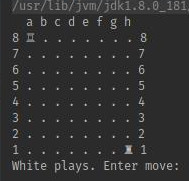
\includegraphics[scale=2.5]{screenshot1}
\end{figure}

Because of the dark theme it appears that the black and white rooks have swapped position from what they should be but I have checked and the correct characters are being printed. When run within a console this will appear correct. \newline

\noindent \textbf{Testing Moving Pieces}

Because of the nature of this code instead of providing screenshots of every single move for every single situation (resulting in a testing section saturated by hundreds of unimportant screenshots). Instead I will describe the situation I am testing and what part of the specification it solves then provide a screenshot of the final result. Below is a screenshot of the start state of the program before I do any tests:
\begin{figure}[H]
\centering
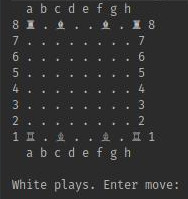
\includegraphics[scale=2.5]{startState}
\end{figure}

The first test I shall perform is moving a rook, I will make the following moves:

\noindent h1, h2,

\noindent a8, a7

\noindent h2, g2

\noindent a7, b7

Essentially I am moving the top left rook one space down and one space to the right and the bottom right rook one move up and one move to the left. The following is the resulting board:
\begin{figure}[H]
\centering
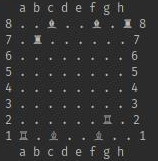
\includegraphics[scale=2.5]{rookBasicMovement}
\end{figure}
As you can see the pieces have moved as expected. This test shows that a rook is able to move up, down, left, and right. Next I need to test that the program will not let the rook move to an invalid space. To do this I attempt the following moves:

\noindent h1, c8
\noindent h1, h1

The result of these moves is the following board:
\begin{figure}[h]
\centering
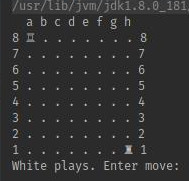
\includegraphics[scale=2.5]{screenshot1}
\end{figure}

This first move tests whether the program will allow you to move somewhere not in the same row or column as the start position and the second move tests whether the program allows you to move a piece to the same original place (which it shouldn't). For both moves the program doesn't change the board and doesn't change who's turn it is, this is reflected by the screen shot above.

The next thing I need to test is how the Rook class deals with obstacles, to do this I shall make the following moves:

\noindent a1, a4

\noindent a8, a1

This is attempting to move the black rook through the white rook which shouldn't be allowed, the result is shown below:
\begin{figure}[h]
\centering
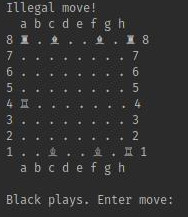
\includegraphics[scale=2.5]{nothingHappened}
\end{figure}

As shown from the screenshot the second move is invalid and will not be made. The final thing I need to test with the Rook class is whether it can "take" other pieces. To do this I shall execute the following moves:

\noindent a1 a8

\noindent h8, h1

\noindent a8, b8

This code is executed so that each player takes the other player's piece and then one moves after to show that the other player's piece has been removed. Below is the result of this: 
\begin{figure}[h]
\centering
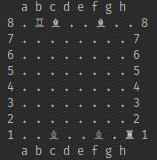
\includegraphics[scale=2.5]{rookTakesRook}
\end{figure}

As you can see each player has taken one of the other players rooks using their rooks and once moved the other player's piece is no longer there. \newline

Now that I have shown the Rook pieces behave as expected I next want to show that the Bishop pieces also work as expected. As with the Rook I want to first show the Bishop pieces can move as expected. To do this I shall execute the following moves:

\noindent c1, a3

\noindent c8, a6

\noindent f1, h3

\noindent f8, h6

I chose to move the pieces in this way as it shows pieces can move in any of the diagonals, the result after these four moves is shown below:
\begin{figure}[h]
\centering
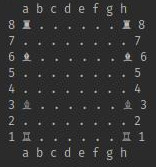
\includegraphics[scale=2.5]{bishopsMoving}
\end{figure}
As you can see the pieces are able to move in all diagonal directions. Next I need to test if the program stops the user making illegal moves. To do this I shall attempt to move in a non-diagonal and attempt to move to the same position using the following moves:

\noindent c1, c7

\noindent f8, f8

The result of this is shown below:
\begin{figure}[h]
\centering
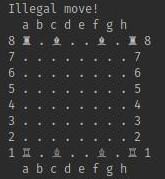
\includegraphics[scale=2.5]{illegal}
\end{figure}

As shown both moves are recognised as invalid and the program doesn't change who's turn it is. The next thing I need to check is whether obstructions are recognised. To do this I will move a rook into the path of a bishop and see if the program recognises this. To do this I will make the following moves:

\noindent a1, a2

\noindent a8, a7

\noindent a2, b2

\noindent a7, b7

\noindent c1, a3

The last move should be recognised as invalid as you are attempting to move the rook through the bishop, below is the board after these moves are made:
\begin{figure}[H]
\centering
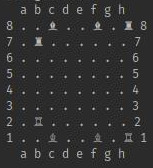
\includegraphics[scale=2.5]{rookObstruction}
\end{figure}

As shown, the program allows all the moves to be made apart from the one that has a Rook obstructing the bishops path. The code for detecting whether the final place is occupied is the same as with the Rook so I will not retest it here. The last thing I want to test is if the user enters nonsense whether the game will recognise an invalid move. In the following table shows the result when I try and make a move whether the program recognises that move as valid or not. (Note: all moves were the first move in the game).
\begin{table}[H]
\begin{tabular}{|l|l|l|}
\hline
\textbf{First Input} & \textbf{Second Input} & \textbf{Valid/Invalid} \\ \hline
a1                   & a8                    & Legal                  \\ \hline
z7                   & z1                    & Illegal                \\ \hline
asdasj               & aijsdiso              & Illegal                \\ \hline
a8                   & a9                    & Illegal                \\ \hline
88                   & 81                    & Illegal                \\ \hline
8a                   & 1a                    & Illegal                \\ \hline
\end{tabular}
\end{table}
First I make a valid move to show the program recognises this. Next I want to check a number of possible invalid moves. The following tests show that the program detects the following possible problems: \begin{itemize}
\item When the letter input is outside the range.
\item When the string inputted is too long.
\item When the number input is too large.
\item When the first character is a number not a letter.
\item When the letter and number are the wrong way round.
\end{itemize}
From these tests I can safely say that the move input is being correctly checked to see if everything is valid. \newline

\noindent \textbf{Testing the Game Loop}
There are a few things I need to test within the game loop: \begin{itemize}
\item Whether the game keeps track of whose turn it is correctly.
\item Whether the game ends when a winning condition is met.
\item Check for the user typing quit.
\end{itemize}

First I shall test whether the game keeps track of whose turn it is. To do this I shall make a series of moves with some being intentionally invalid. I will show the game deals with this appropriately:
\begin{table}[H]
\begin{tabular}{|l|l|l|}
\hline
\textbf{Player's Turn Before Move} & \textbf{Was The Move Legal?} & \textbf{Player's Turn After Move} \\ \hline
White                              & Yes                          & Black                             \\ \hline
Black                              & Yes                          & White                             \\ \hline
White                              & No                           & White                             \\ \hline
White                              & Yes                          & Black                             \\ \hline
Black                              & No                           & Black                             \\ \hline
\end{tabular}
\end{table}
As you can see from the first two moves, when a legal move is made the program recognises this and switches the turn. The next line shows that if white makes an illegal move then the program will not switch turns, the last line shows that if black makes an illegal move the game will also not switch turns. From these tests I can therefore safely say that the game keeps track of whose turn it is. The way I determined which player had their turn was the output prompting the user for a move. Below are screenshots of each message.
\begin{figure}[H]
\centering
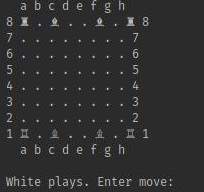
\includegraphics[scale=2.5]{whitePlays}
\end{figure}
\begin{figure}[H]
\centering
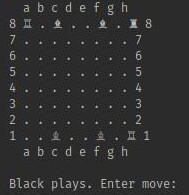
\includegraphics[scale=2.5]{blackPlays}
\end{figure}

The next thing I am going to test is whether the game recognises a winning game state and reacts appropriately. To do this I shall two games, one where white wins and another where black wins. I will show the resulting boards and the message shown. Firstly the below image shows the state of the board after white takes all the black pieces.
\begin{figure}[H]
\centering
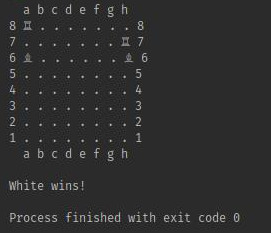
\includegraphics[scale=2.5]{whiteWins}
\end{figure}

From this I can see that the program that when there are no black pieces left, the program recognises this as a white win and stops the program. Next I need to do the same for a black win. The resulting board is shown below.
\begin{figure}[H]
\centering
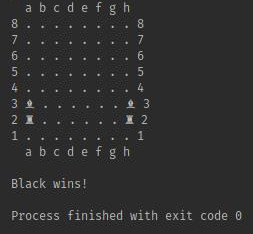
\includegraphics[scale=2.5]{blackWins}
\end{figure}

The next and final thing I want to show is that the program exits when the user types quit. Below is the screenshot of this happening.
\begin{figure}[H]
\centering
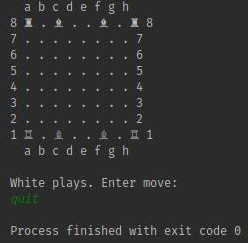
\includegraphics[scale=2.5]{quit}
\end{figure}

\section*{Evaluation}
In the specification I was asked to create a version of chess where each player had two rooks and two bishops. The game should end when either player has taken all the other player's pieces. In my game the board appears as expected by the specification with all the pieces in the right spots at the start of the game. The players are able to make moves when it is their turn by typing the start and end coordinates of their move. The program then correctly identifies which moves are valid or invalid and makes the move if the move is valid. If the move is invalid the game prompts the user to enter another move. The game stops when either player takes all the other player's pieces and outputs a correct winning message depending on which player wins as expected by the specification. The player can quit the game mid-match by typing the word quit at any point. As described in this paragraph the program has all the functionality expected by the specification.

\section*{Conclusion}
During the development of my solution I was able to achieve a number of things. First and foremost I was able to take advantage of object orientation in a way that I haven't been in previous projects. Namely, I was able to use an abstract class for ChessPiece and have the Rook and Bishop classes inherit from this. Because of the use of abstraction I was able to have one polymorphic array to iterate through all the ChessPiece objects which reduced code reuse and made development significantly faster. It also means that my extension will be easier to develop as I can write objects for all the other pieces which can inherit from ChessPiece.

Another thing I was able to achieve was the use of both static and dynamic data structures. I used a static data structure to store the characters on the board as a 2D array. I chose to use a static data structure for this purpose as the board size doesn't change during execution. To store the pieces on the board I chose to use a list, which is a dynamic data structure, as the amount of pieces on the board changes during execution.

Another feature of object orientation I was able to use was encapsulation. I kept almost all of the attributes of classes private and used public methods to access them. This meant that I could ensure the values that were being assigned were valid to avoid bugs in the game. This is most evident when the user enters a move as the program has to do a lot of checks to assure that the move is valid, public methods are used to do this as it makes sure the user cannot cause any bugs.

There were a few things I found particularly tricky during development, one of them was checking if a move was valid for a bishop as it was quite difficult to figure out how to check efficiently if there was pieces in the way. I drew some diagrams by hand to work this out and eventually got a solution which worked well.

During my extension there are a few things I want to add that were not in the original specification. I want to add all the other pieces in chess to the board and change the win-state to be when either player has a checkmate as with traditional chess. Finally I want to add the option to play against an AI. I could also improve the program by adding more helpful error messages for what is invalid about any particular move.

\section*{Extension}
\section*{Overview}
For my extension, I aim to implement an almost complete version of chess with a simple AI to play. This would involve the implementation of the following: \begin{itemize}
\item Add all the other chess pieces.
\item Write code to detect check and checkmate.
\item Write an AI.
\end{itemize}
\section*{Design}
The first thing I wished to add in my extension was the other pieces in chess. The first piece I decided to add was the Queen. The code for the queen is pretty simple, to check if a move is valid it makes two temporary pieces with the same x and y coords and then checks if the same move would be valid for either of those pieces.

The code for the King was slightly more complex. To check if a move is within the valid squares, I check that both the x and y coordinates are not more than 1 less or more than the original x and y coordinates and that the piece has actually moved in the first place, then I do a check on the final position to see if the position is occupied and to take any opposite pieces there.

The code for the Knight was difficult to design as the logical tests weren't easy to come up with. Eventually I settled on a logical statement that detects whether a set of coordinates are valid by checking that only one of the x or y coordinates increase or decrease by 2 while the other y or x coordinate increases or decreases by 1. Then as with the other pieces I need to do checks on whether there are any pieces in the final space.

The code for the Pawn was probably the most complex as there are lots of different kind of moves that can be performed by a Pawn.  Firstly a pawn can either move one or two moves forward - but only two moves if it is that pawns first time moving. The pawn cannot take pieces in the same column as itself rather can move one place forward diagonally to take a piece. This meant lots of logical tests were needed to detect what kind of move the player was making.

There are a number of other rules in chess I chose not to implement for sake of simplicity like castling, and pawn promotion. Instead I wanted to focus on programming an AI for this simplified version of chess. The first thing I needed to program was a different win condition. In this version of chess you do not win by taking every other piece, instead you win by creating a checkmate. That is a situation where the opponent cannot make a move that would put their King in a position it cannot be taken. This means I need to be able to check for checks  and checkmates and let the player know.

One of the more difficult tasks was looking for a check or checkmate. The way I did this was have a method that gets all the possible boards that could occur from a given player's turn. I would then iterate through this list and see if in any of the boards a king was missing. This means a check exists and whichever player's turn you were checking for had a check. The checkmate test was harder to design. To do this I iterate through all the moves the opponent can do and see if any of them are not a check state.

The last thing I had to program was the AI. To program the AI I first assigned a "score" to each ChessPiece subclass. With higher points representing more important pieces. The AI then forms a tree of possible boards and then performs a min max algorithm to find the best possible move based on the score.

\section*{Testing}

\noindent \textbf{Testing Movement of New Pieces}

Before I test how the game works as a whole I will first test the movement code of each piece. To do this I will create a piece and then try moving it to every place on the board and see if the game correctly identifies the valid moves.

First I will test the Queen. The board starts in this state: 
\begin{figure}[H]
\centering
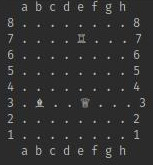
\includegraphics[scale=2.5]{queenStartPos}
\end{figure}

I will then iterate and print a 1 for places the queen can move and print a 0 for unavailable spots. The following output is shown:
\begin{figure}[H]
\centering
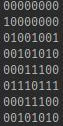
\includegraphics[scale=2.5]{queenPosMoves}
\end{figure}
As shown by the image the Queen is able to move in all diagonals and horizontally and vertically unless obstructed by a piece. It also knows it can take the piece that is the opposite colour. The code to actually perform the moves is the same as with the non-extension code so I shall not test it again.

Next I shall test the possible moves for the King. I will do the same thing but replace the Queen piece with a King. The start position is shown below:
\begin{figure}[H]
\centering
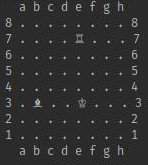
\includegraphics[scale=2.5]{kingStartPos}
\end{figure}

The possible move array is shown below:
\begin{figure}[H]
\centering
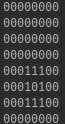
\includegraphics[scale=2.5]{kingPosMoves}
\end{figure}

The King exhibits the expected behaviour and is only able to move to adjacent places so passes the test.

Next I will test the Knight, below is the starting board for the test: 
\begin{figure}[H]
\centering
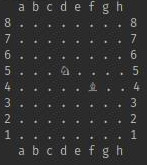
\includegraphics[scale=2.5]{knightStartPos}
\end{figure}

The possible move array is shown below: 
\begin{figure}[H]
\centering
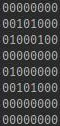
\includegraphics[scale=2.5]{knightPosMoves}
\end{figure}

The knight exhibits the expected behaviour and doesn't move onto the piece from the same team. From this I can say that the Knight class passes the test.


Finally I will test for a pawn, to test all the possible conditions I will start with the following board:
\begin{figure}[H]
\centering
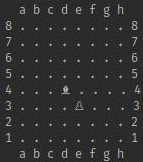
\includegraphics[scale=2.5]{pawnStartPos}
\end{figure}

The possible move array is shown below:
\begin{figure}[H]
\centering
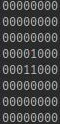
\includegraphics[scale=2.5]{pawnPosMoves}
\end{figure}
As you can see the pawn can either move one move up, two moves up (as it is the pawns first move) or take the piece diagonally adjacent. This is as expected so I can say that the test is passed. \newline

\noindent \textbf{Testing Check and Checkmate}

This is quite tricky to test as there are an extremely large number of situations that could be known as check or checkmate. For the sake of simplicity I will show that the game works for one example of a check and one example of a checkmate. Below is an example of a check: 
\begin{figure}[H]
\centering
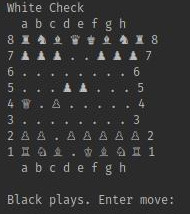
\includegraphics[scale=2.5]{check}
\end{figure}

From the text at the top you can see the game is notifying the player of a check. Its a check and not a checkmate as the other play can move to get out. Below is an example of a checkmate:
\begin{figure}[H]
\centering
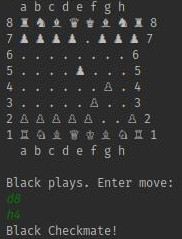
\includegraphics[scale=2.5]{checkMate}
\end{figure}

As you can see the d8 to h4 move would place the queen in a position to take the king and the king wouldn't be able to move. The program has successfully detected the checkmate and stopped the execution of the program. \newline

\noindent \textbf{Testing the AI}

I attempted to make an AI using the minmax algorithm with alpha-beta pruning but I've been yet to figure out why it doesn't work. It plays moves that are sometimes as expected but are often very rubbish. The algorithm often finds itself unable to escape checks. 

\section*{Evaluation}

At the start of developing my extension I said I wanted a slightly simplified version of chess with an AI. I was successfully able to add the other pieces in chess and have them move as expected, I was also able to test the board for checks and checkmates as a winning condition instead of when all the other pieces are taken. The one thing I had a problem with was developing an AI. I managed to make a class, ComputerPlayer, that makes moves. Often the AI makes a stupid move or cannot escape chess. I used a minmax alpha-beta pruning algorithm.

\section*{Conclusion}

As with the starter I was able to use a lot of the aspects of Object-Oriented programming during the development of this program. I was able to further extend the ChessPiece class with the Pawn, Knight, Queen, and King classes all with their own implementation of ChessPiece's abstract methods. These methods could then be used by a group of methods used to determine whether a check or checkmate exists and to find the possible moves. The ability to get possible moves was used by the "AI" to find its next move.

I found the AI very difficult to debug. The recursive nature of its methods made this so as there were so many branches to check that I couldn't get my head around figuring out what was wrong. If given more time I would try and fix this but I am at the point in the development where I think a full rewrite would be the only solution to figure out exactly what is happening and that would erase all the other progress I've made.

\end{document}